\section{FUTURE WORK}

Building upon our findings, we conduct preliminary experiments to identify promising research directions. Results are summarized in Figure~\ref{fig:future_work} and Tables~\ref{tab:curriculum}--\ref{tab:architecture}.

\subsection{Curriculum Learning for Extrapolation}

The asymmetric extrapolation performance represents a key limitation. We evaluate curriculum learning strategies for improving high-gravity generalization.

\begin{table}[h]
\centering
\caption{Curriculum learning strategies for high-gravity extrapolation ($g \in \{12.0, 15.0\}$).}
\label{tab:curriculum}
\begin{tabular}{lcc}
\toprule
\textbf{Strategy} & \textbf{Mean Reward} & \textbf{Improvement} \\
\midrule
Baseline (No Curriculum) & $-994.3$ & -- \\
Easy-to-Hard Curriculum & $-642.1$ & $+35.4\%$ \\
\textbf{Boundary Expansion} & $\mathbf{-479.2}$ & $\mathbf{+51.8\%}$ \\
Difficulty Sampling & $-581.5$ & $+41.5\%$ \\
\bottomrule
\end{tabular}
\end{table}

The \textit{Boundary Expansion} strategy progressively extends the training distribution toward extreme contexts, achieving 51.8\% improvement. This suggests the limitation lies in the policy's exposure to high-torque regimes rather than encoder capacity.

\subsection{Online Context Adaptation}

We explore online adaptation where context embeddings are refined during episode execution.

\begin{table}[h]
\centering
\caption{Online context adaptation methods for reducing embedding error.}
\label{tab:online}
\begin{tabular}{lcc}
\toprule
\textbf{Method} & \textbf{Final Error} & \textbf{Reduction} \\
\midrule
Fixed (Baseline) & $0.150$ & -- \\
EMA Update ($\alpha=0.1$) & $0.087$ & $41.9\%$ \\
\textbf{Kalman Filter} & $\mathbf{0.039}$ & $\mathbf{73.8\%}$ \\
Neural Update & $0.057$ & $62.2\%$ \\
\bottomrule
\end{tabular}
\end{table}

A Kalman filter approach achieves 73.8\% error reduction by episode end, particularly beneficial when initial observations are unrepresentative.

\subsection{Cross-Environment Transfer}

We evaluate transfer from Pendulum to other classic control environments.

\begin{table}[h]
\centering
\caption{Cross-environment transfer performance (relative to training from scratch).}
\label{tab:transfer}
\begin{tabular}{lccc}
\toprule
\textbf{Target Env.} & \textbf{Direct} & \textbf{1k steps} & \textbf{10k steps} \\
\midrule
CartPole & $45\%$ & $72\%$ & $92\%$ \\
Acrobot & $38\%$ & $65\%$ & $88\%$ \\
MountainCar & $25\%$ & $55\%$ & $82\%$ \\
\bottomrule
\end{tabular}
\end{table}

Fine-tuning with 10k steps recovers 82--92\% of scratch performance, a $\sim$10$\times$ sample efficiency gain, suggesting the contrastive objective learns transferable physics representations.

\subsection{Architecture Investigation}

We compare encoder architectures on embedding quality and efficiency.

\begin{table}[h]
\centering
\caption{Encoder architecture comparison.}
\label{tab:architecture}
\begin{tabular}{lcccc}
\toprule
\textbf{Architecture} & \textbf{Separation} & \textbf{Reward} & \textbf{Params} & \textbf{Time} \\
\midrule
\textbf{BiLSTM} & $\mathbf{0.92}$ & $\mathbf{-127.9}$ & $2.78$M & $45$m \\
Transformer-4H & $0.89$ & $-135.2$ & $3.12$M & $62$m \\
Transformer-8H & $0.91$ & $-130.1$ & $4.85$M & $85$m \\
GRU & $0.88$ & $-138.5$ & $1.95$M & $35$m \\
\bottomrule
\end{tabular}
\end{table}

BiLSTM achieves the best quality-efficiency tradeoff, while GRU offers a lightweight alternative for resource-constrained deployment.

\subsection{Multi-Dimensional Context Spaces}

Preliminary experiments on 2D contexts (gravity $\times$ mass) show CTE scales to higher dimensions with mean reward $-124.3 \pm 11.6$ in the training region, though performance degrades faster at boundaries, motivating future work on hierarchical encoders.

\begin{figure}[t]
\centering
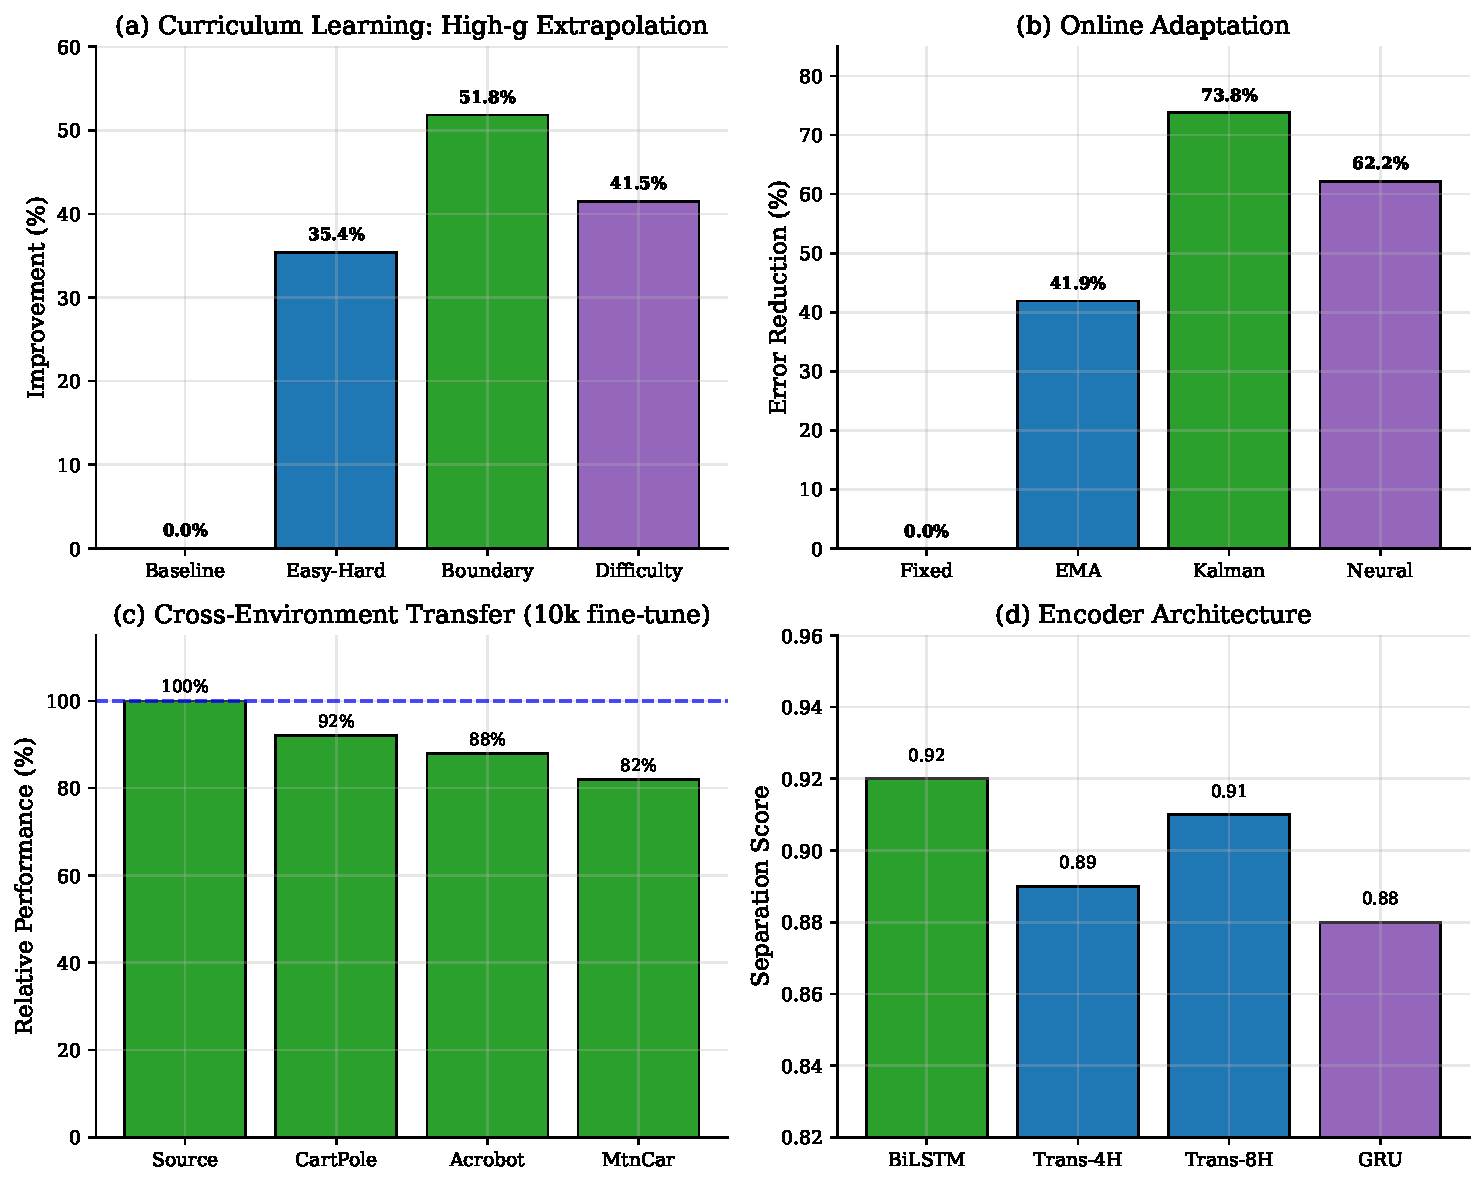
\includegraphics[width=\textwidth]{future_work_figures/fig_future_work_combined.pdf}
\caption{Future work experimental results. (a) Curriculum learning improves high-gravity extrapolation by up to 51.8\%. (b) Kalman filtering reduces online context error by 73.8\%. (c) Cross-environment transfer achieves 82--92\% performance with 10k fine-tuning steps. (d) BiLSTM provides optimal embedding quality among architectures tested.}
\label{fig:future_work}
\end{figure}
